\documentclass{article} % For LaTeX2e
\usepackage[final]{colm2026_conference}

\usepackage{microtype}
\usepackage[table]{xcolor}
\usepackage{hyperref}
\usepackage{url}
\usepackage{booktabs}
\usepackage{graphicx}
\usepackage{tabularx}
\usepackage{array}
\usepackage{capt-of}
\usepackage{enumitem}
\setlist{nosep}
\setlength{\textfloatsep}{8pt plus 2pt minus 2pt}
\setlength{\floatsep}{6pt plus 2pt minus 2pt}
\setlength{\abovecaptionskip}{4pt}
\usepackage[capitalise]{cleveref}
\crefname{table}{Tab.}{Tabs.}
\crefname{figure}{Fig.}{Figs.}
\crefname{section}{Sec.}{Secs.}

\definecolor{darkblue}{rgb}{0, 0, 0.5}
\hypersetup{colorlinks=true, citecolor=darkblue, linkcolor=darkblue, urlcolor=darkblue}
\definecolor{labours}{HTML}{EDEDED}
\newcommand{\ci}[2]{{\scriptsize[#1, #2]}}
\newcommand{\pmstd}[2]{#1{\scriptsize\,$\pm$\,#2}}
\newcolumntype{L}[1]{>{\raggedright\arraybackslash}p{#1}}
\newcolumntype{Y}{>{\raggedright\arraybackslash}X}

\title{Homework 3: Adding complexity to MLP probes improve activation classification}

\author{Khai-Nguyen Nguyen, University of Virginia \\
\url{https://github.com/nkn002/visual-readout}}

\begin{document}

\maketitle
\lhead{DS 7400 Deep Learning, Homework 3 experiment report}

\begin{figure}[!ht]
\centering
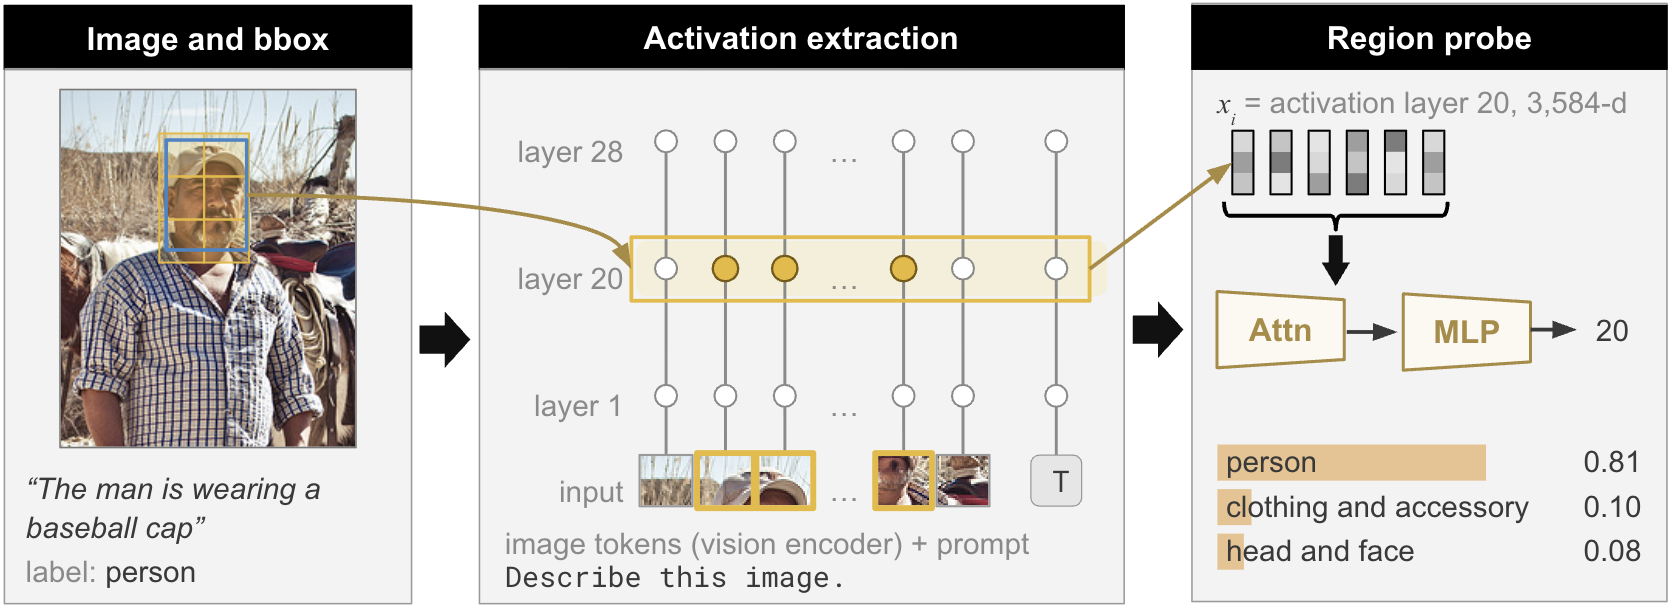
\includegraphics[width=\textwidth]{fig_mechanism.png}
\caption{Our work trains a probe that reads the frozen Qwen2.5-VL-7B-Instruct's activations layer 20 at the $L$ tokens within the yellow the box.}
\label{fig:mech}
\end{figure}

\section{Hypothesis}
\label{sec:hyp}

\textbf{Problem.} In Homework 2, we trained an MLP probe \citep{alain2017understanding} (3584 $\to$ 512 $\to$ ReLU $\to$ 20) to classify a region's activation into one of 20 object categories.
For each Visual Genome bounding box \citep{krishna2017visual} we extract its corresponding activation from layer-20 of Qwen2.5-VL-7B-Instruct \citep{qwen2025qwen25technicalreport}. The probe input vector is the mean-pooled activation of the image tokens corresponding to this box (\cref{fig:mech}).
This MLP probe reaches only 73.62\% test accuracy.
We hypothesize that mean pooling causes part of this error, as it weights every token under the box equally.


\textbf{Proposed solution.} We replace the mean pooling vector with single-headed attention pooling, $\sum_i a_i x_i$ with $a_i = \mathrm{softmax}_i\big(q^\top W_k \hat{x}_i / \sqrt{64}\big)$ over the standardized tokens $\hat{x}_i$. We also evaluate a 8-headed attention pooling variant to observe if performance improve with added complexity.

\textbf{Predictions.} Our design is motivated by our hypothesis that trained attention weights learns to focus on relevant activations corresponding to the main object in the bounding box. We expect the following:
\begin{enumerate}
    \item Accuracy does not change on one-token boxes, as attention pooling returns the same vector as mean pooling.
    \item Accuracy improvement via attention-pooling grow with box size as attention-pooling enables the model to focus on more relevant activations.
    \item Adding a second hidden layer to the probe improves classification accuracy due to extra capacity.
    \item Similarly, 8-head attention pooling beat 1-head attention pooling with extra capacity.
\end{enumerate}



\section{Experimental Setup}
\label{sec:setup}

We trained the proposed design of activation probes on the HW2 split: 50,000 regions, 2,500 per category, split by image into 39,968 train, 5,075 validation, and 4,957 test regions. We use Adam optimizer with grid search hyperparameter tuning (learning rate \{3e-4, 1e-3\} $\times$ weight decay \{1e-4, 1e-3\}). We keep the best setting based on validation accuracy, and reruns it with 3 seeds.


\section{Results}
\label{sec:results}



\textbf{Prediction 1 holds for 1-head attention pooling but not for eight heads.}
On one-token boxes, one-head attention gains +0.08\% over HW2, as expected (\cref{fig:bins}).
Interestingly, eight heads gain +1.30\% on the same boxes.
We hypothesize that part of the eight-head gain comes from the jointly trained MLP or from seed variance (HW2's seeds span 73.09\% to 73.90\%), not from the attention re-weighting the tokens.

\begin{table}[t]
\centering
\caption{Eight heads with 2 hidden layers reach the best test accuracy, 75.07\% (HW2 probe, top left: 73.62\%). Cells give test accuracy (\%) as mean $\pm$ std over 3 seeds; each $\Delta$ is a gain in\% with its 95\% paired-bootstrap CI.}
\label{tab:main}
\small
\setlength{\tabcolsep}{5pt}
\begin{tabular}{@{}lccc@{}}
\toprule
Pooling & 1 hidden layer & 2 hidden layers & $\Delta$ second layer \\
\midrule
Mean pool & \pmstd{73.62}{0.38} & \pmstd{74.10}{0.21} & +0.48 \ci{+0.01}{+0.95} \\
Attention, 1 head & \pmstd{74.10}{0.15} & \pmstd{74.33}{0.08} & +0.23 \ci{$-$0.29}{+0.71} \\
Attention, 8 heads & \pmstd{74.48}{0.17} & \pmstd{\textbf{75.07}}{0.25} & +0.59 \ci{+0.09}{+1.06} \\
\bottomrule
\end{tabular}
\end{table}

\begin{figure}[!ht]
\centering
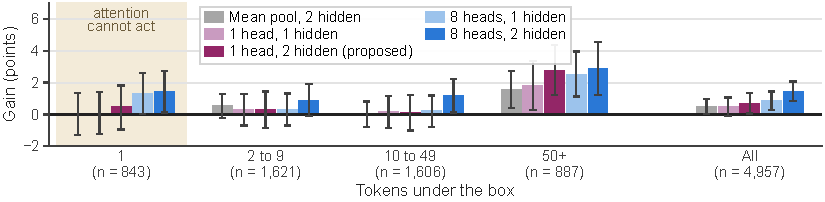
\includegraphics[width=\textwidth]{fig_gain_by_box_size.pdf}
\caption{Eight heads gain +1.30\% on one-token boxes, where attention cannot have any effect (shaded). Single headed attention pooling gains +0.08 there and +1.80 on boxes with 50+ tokens.}
\label{fig:bins}
\end{figure}

\textbf{Prediction 2 holds only for the largest boxes.}
1-head attention gains at most +0.29\% on boxes of 2 to 49 tokens and +1.80 on boxes of 50 or more (\cref{fig:bins}).
That is, the gain does not grow steadily with box size, it appears only in the last bin.
Furthermore, the mean pool with 2 hidden layers gains +1.54 on these large boxes, so the gain is not specific to attention.

\textbf{Prediction 3 holds: a second hidden layer improves the mean-pool probe.}
The mean pool with 2 hidden layers reaches 74.10\%, +0.48\% over HW2 probe (\cref{tab:main}).
This depth gain accounts for most of the proposed design's +0.71.
One-head attention adds only +0.24 on top of the same depth.

\textbf{Prediction 4 holds: eight heads match or beat one head.}
Eight heads gain +0.73\% over one head with 2 hidden layers and +0.38 with 1 hidden layer (\cref{tab:main}).
The best arm (8 heads, 2 hidden layers) reaches 75.07\%, +1.45 over HW2.
However, part of this gain appears on one-token boxes (prediction 1), so we cannot attribute all of it to attention.

\section{Conclusion}

Adding capacity to the HW2 probe improves test accuracy: the best probe (8-head attention pooling, 2 hidden layers) reaches 75.07\%, +1.45\% over HW2.
A second hidden layer (+0.48\% on the mean pool) and eight attention heads (+0.73\% over one head, with 2 hidden layers) both contribute. However, our results do not show that attention helps by focusing on the relevant tokens. Instead, extra capacity leads to this accuracy improvement, consistent with the scaling law \citep{kaplan2020scalinglawsneurallanguage} of neural networks.



\bibliographystyle{colm2026_conference}
\bibliography{colm2026_conference}

\end{document}
